\cleardoublepage

\chapter{Casos de Estudio}
\label{makereference6}

Partiendo de un prototipo operativo de suite domótica, podemos abordar el caso de uso planteados en el capitulo 1 sección de objetivos. El escenario se desarrolla en una bodega de uso domestico situado bajo tierra. El acceso a la misma se encuentra dentro de un hogar a través de unas escaleras que bajan hasta la estancia donde una pareja de toneles fermentan vino de cosecha propia de la unidad familiar que reside en la casa. Originalmente este espacio había sido diseñado como almacén y no dispone de medios electrónicos salvo el cableado de iluminación que dispone de un interruptor en la parte superior de las escaleras.

Existe una serie de condiciones previstas para una buena conservación del vino embotellado en una bodega , humedad relativa de tu bodega debe estar entre el 65 por ciento y el 75 por ciento . En una bodega demasiado seca pueden llegar a resecarse los tapones, mientras que una excesivamente húmeda presenta el peligro de que se alteren los tapones y las etiquetas debido a la aparición de mohos.
La temperatura oscilará entre los 10-15°C y será, en lo posible, constante; por otra parte, debe estar bien ventilada pero sin grandes corrientes de aire. Una bodega demasiado fresca ralentiza la evolución del vino y puede ser la causa de que se produzca la precipitación de cristales de tartratos. Por el contrario, en una bodega en la que la temperatura es demasiado alta, el vino tiende a evolucionar más rápidamente y esto puede llegar a traducirse en un envejecimiento prematuro

Descargamos la paquetería de Adafruit para el primer sensor de pruebas, el sensor DTH11 de temperatura y humedad.
Se requiere un montaje sencillo.
\begin{figure}[hbt!]
\centering
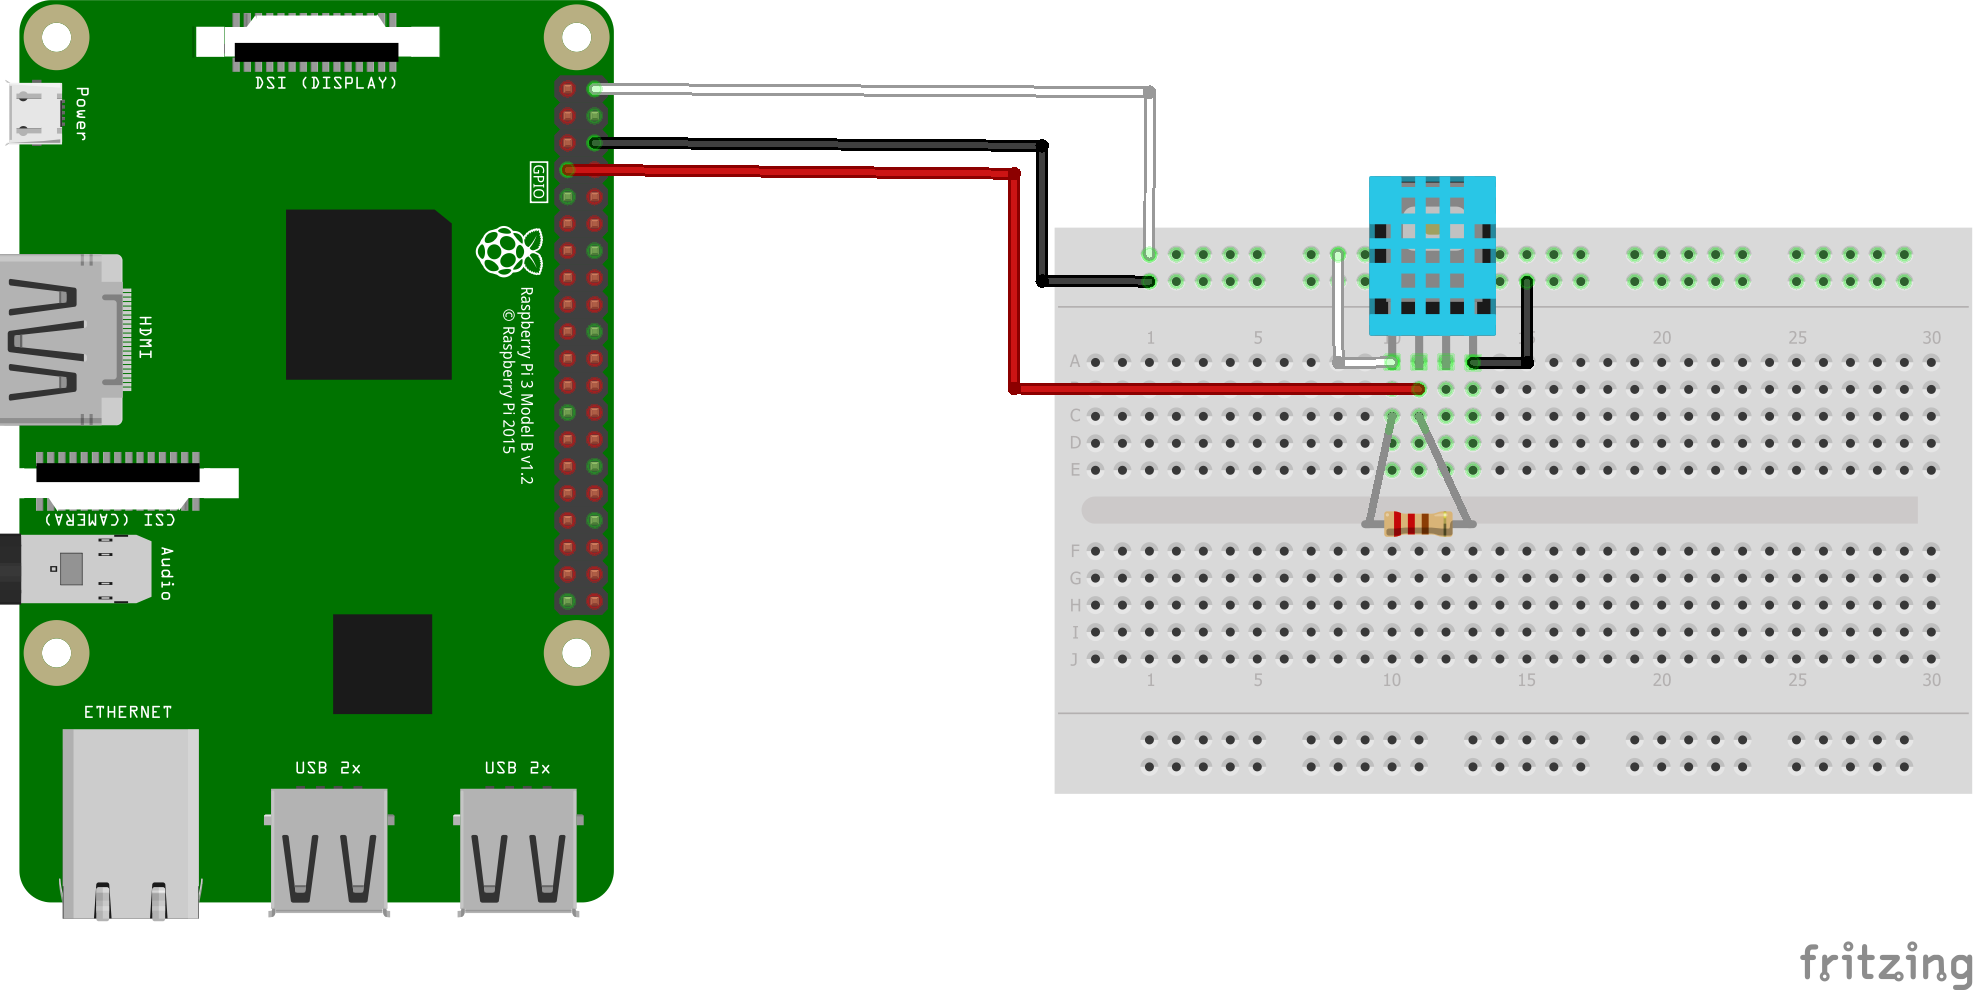
\includegraphics[height=2.5in]{figures/nodo_1.png}
\end{figure}

Clonamos la librería del sensor, nos ubicamos en la ruta descargada \verb|cd Adafruit_Python_DHT| e instalamos la librería \verb|sudo python setup.py install|, previamente instalamos las dependencias de la librería para su instalación \verb|sudo apt-get install python-setuptools| considerando que tenemos la versión de python 2.7.3, esto permitirá instalar la librería de python para el sensor DHT version 1.4. Se debe realizar una prueba de contacto con un script que nos muestre la información por pantalla para verificar que las conexiones del sensor a la rapsberry son correctos. Este primer script es un bucle infinito de mediciones de temperatura y humedad cada poco segundos. Hay una justificación para elegir un bucle sobre una única medida del sensor y está fundamentada en el margen de error inicial de las medidas. Si bien el sensor DTH11 es una opción muy común por su bajo coste y facilidad de implementación (este sensor se caracteriza por tener la señal digital calibrada por lo que asegura una alta calidad y una fiabilidad a lo largo del tiempo, ya que contiene un microcontrolador de 8 bits integrado. Está constituido por dos sensores resistivos (NTC y humedad) - revisar esta info y contrastarla contra ésta: \url{ https://programarfacil.com/blog/arduino-blog/sensor-dht11-temperatura-humedad-arduino/}), ademas de manejar señales digitales que no se ven afectadas por las fluctuaciones de voltaje, tiene algunas contrapartidas que deben tenerse en cuenta. Se necesita un tiempo mínimo de espera entre medidas (de al menos 1 segundo), hecho que no agrava particularmente su desempeño en entornos cerrados como una casa, ya que las variaciones de temperatura y humedad no son bruscas, aun así existen estrategias para reducir estos tiempos, por ejemplo, usar la función millis() de Arduino, el cual nos da el tiempo en milisegundos desde que empieza a ejecutarse el código, De esta forma evitamos la pausa de los 2 segundos, pero no el tiempo que demora en hacer la lectura, que es de aproximadamente  250 milisegundos, el cual lo pueden notar si realizan el ejemplo anterior, en donde se hace parpadear el led interno de la placa (Pin 13) con pausas de 100ms (tomado de \url{https://naylampmechatronics.com/blog/40_Tutorial-sensor-de-temperatura-y-humedad-DHT1.html}). Otro problema que abordar es que las primeras lecturas tienen un margen de error de unos +-2 grados Celsius y +-5\% de humedad relativa en las primeras 4 lecturas. Esto generará un problema a la hora de tomar lecturas instantáneas si el sensor no se encuentra ya operando cuando se solicita el dato. Como estrategia, haremos que el sensor tome medidas indefinidamente y los vuelque en un fichero/BBDD para recortar los tiempo de respuesta, evitando así esperar a que el sensor haga la toma de medidas en el momento+ de solicitud y sacándolas en su lugar del último registro que tengamos. Un último problema con el que hay que lidiar es su baja precisión limitada a enteros, por lo que no podemos esperar obtener un dato preciso a la décima de la temperatura y humedad. Esto sin embargo no es un problema real dada la naturaleza del proyecto, ya que no necesitamos un grado de precisión menor a la unidad para tomar acciones o informar al usuario.
